\documentclass[UTF8]{ctexart}

%固定图片位置
\usepackage{float}

%插入超链接
\usepackage{url}

\usepackage{tikz,mathpazo}
\usetikzlibrary{shapes.geometric, arrows}
\usetikzlibrary{calc}

%\usepackage[affil-it]{authblk}

\usepackage{listings}
%插入代码的配置
\definecolor{CPPLight}  {HTML} {686868}
\definecolor{CPPSteel}  {HTML} {888888}
\definecolor{CPPDark}   {HTML} {262626}
\definecolor{CPPBlue}   {HTML} {4172A3}
\definecolor{CPPGreen}  {HTML} {487818}
\definecolor{CPPBrown}  {HTML} {A07040}
\definecolor{CPPRed}    {HTML} {AD4D3A}
\definecolor{CPPViolet} {HTML} {7040A0}
\definecolor{CPPGray}  {HTML} {B8B8B8}
\lstset{
	language=Matlab,                                     % 设置语言
    columns=fixed,    
    breaklines = true,   
    basicstyle=\small ,
    numbers=left,                                        % 在左侧显示行号
    %frame=none,                                          % 不显示背景边框
    backgroundcolor=\color[RGB]{245,245,244},            % 设定背景颜色
    keywordstyle=\color[RGB]{40,40,255}\bfseries,                 % 设定关键字颜色
    %commentstyle=\color{red!10!green!70}\textit,    % 设置代码注释的颜色
    numberstyle=\tiny\color{darkgray},           % 设定行号格式
    commentstyle=\it\color[RGB]{0,96,96},                % 设置代码注释的格式
    stringstyle=\rmfamily\slshape\color[RGB]{128,0,0},   % 设置字符串格式
    showstringspaces=false,                              % 不显示字符串中的空格                           
    %morekeywords={True,alignas,continute,friend,register,true,alignof,decltype,goto,
    %reinterpret_cast,try,asm,defult,if,return,typedef,auto,delete,inline,short,
    %typeid,bool,do,int,signed,typename,break,double,long,sizeof,union,case,
    %dynamic_cast,mutable,static,unsigned,catch,else,namespace,static_assert,using,
    %char,enum,new,static_cast,virtual,char16_t,char32_t,explict,noexcept,struct,
    %void,export,nullptr,switch,volatile,class,extern,operator,template,wchar_t,
    %const,false,private,this,while,constexpr,float,protected,thread_local,
    %const_cast,for,public,throw,std,rand},
    emph={access,and,break,class,continue,def,del,elif ,else,%
	except,exec,finally,for,from,global,if,import,in,i s,%
	lambda,not,or,pass,print,raise,return,try,while, imshow, subplot, figure,%
    log, fft2, fftshift, abs, size, rgb2gray, imread},
    emphstyle=\color{CPPViolet}\bfseries, 
    emph={[2]True, False, None, self},
	emphstyle=[2]\color{green},
	emph={[3]from, import, as},
	emphstyle=[3]\color{blue},
	upquote=true,
	morecomment=[s]{"""}{"""},
    morecomment=[s]{\%}{},
	%commentstyle=\color{orange}\slshape,
    commentstyle=\color{red!10!green!70}\textit,    % 设置代码注释的颜色
	emph={[4]1, 2, 3, 4, 5, 6, 7, 8, 9, 0},
	emphstyle=[4]\color{red},
	emph={[5]numpy, np, plt},
	emphstyle=[5]\color{red},
	literate=*{:}{{\textcolor{blue}:}}{1}%
	{=}{{\textcolor{blue}=}}{1}%
	{-}{{\textcolor{blue}-}}{1}%
	{+}{{\textcolor{blue}+}}{1}%
	{*}{{\textcolor{blue}*}}{1}%
	{!}{{\textcolor{blue}!}}{1}%
	{(}{{\textcolor{blue}(}}{1}%
	{)}{{\textcolor{blue})}}{1}%
	{[}{{\textcolor{blue}[}}{1}%
	{]}{{\textcolor{blue}]}}{1}%
	{<}{{\textcolor{blue}<}}{1}%
	{>}{{\textcolor{blue}>}}{1},%
    %{\%}{{\textcolor{green}\%}}{1},%
	framexleftmargin=0.1mm, framextopmargin=0.1mm, frame=shadowbox, rulesepcolor=\color{black},
}



\usepackage{geometry}
\geometry{left=2cm, right=2cm, top=1.2cm, bottom=1.2cm}

%得到引用的标题内容
\usepackage{nameref} 

%添加首行缩进,两个字符
\usepackage{indentfirst}
\setlength{\parindent}{2em}

%多行公式一个编号
\usepackage{amsmath}

%文献引用,标准类型为plain
%\usepackage[hyperref=true,backend=biber,sorting=none,backref=true]{biblatex}
%\addbibresource{ref.bib}
\bibliographystyle{plain}
\usepackage{cite}

\pagestyle{plain}

%跨页表格
\usepackage{multirow}
\usepackage{longtable,booktabs}
\usepackage{supertabular}
\usepackage{makecell}

%调整itemize等的间距
\usepackage{enumitem}


\usepackage{graphicx}
\usepackage{subfigure}

%超链接
\usepackage[linkcolor=yellow,citecolor=red,backref=page,hyperfootnotes=true]{hyperref}
\hypersetup{
bookmarks=true,
colorlinks=true,
linkcolor=black
}
\usepackage{tabularx} %This package must be placed after package {hyperref}, otherwise footnote marks are NOT treated as hyperlinks.


%引入了一些改进的数学环境,如align
\usepackage{amsmath}

\title{数字图像处理报告九:图像压缩}
\author{姓名:鲁国锐 \protect\newline
\and 学号:17020021031 \\
\and 专业:电子信息科学与技术}


\begin{document}
	\maketitle
	\renewcommand{\contentsname}{目录}
	\renewcommand{\listfigurename}{插图目录}
	\renewcommand{\listtablename}{表格目录}
	\renewcommand{\refname}{参考文献}
	\renewcommand{\abstractname}{摘要}
	\renewcommand{\indexname}{索引}
	\renewcommand{\tablename}{表}
	\renewcommand{\figurename}{图}
	
	
	
	\tableofcontents
	\newpage
	
	\hypersetup{
	bookmarks=true,
	colorlinks=true,
	linkcolor=red,
	urlcolor=blue
	}
    
    
	\section{题目描述}
	\indent 简单描述$JPEG2000$的图像压缩原理,并与基于深度学习的图像压缩方法进行对比。

			
    \section{$JPEG2000$}
        
        \subsection{原理简述}
    
        \indent $JPEG$是“使用最为普遍且广泛的连续色调静止帧压缩标准”\cite{digit_image_Gonzalez}。但随着今年来人们对于多媒体图像资料需求的增长,旧的标准已难以适应新的潮流,于是促使人们又在其基础上进行扩充,得到了$JPEG2000$标准。该标准共有$8$个部分,其中$PART\ 1$在$2000$年$12$成为了国际标准,其余部分由于知识产权等原因暂未得到推广。故本节只简要介绍$PART\ 1$的压缩流程和原理。
        
        \indent $JPEG2000$标准$PART\ 1$的压缩过程大致可分为以下几步\cite{liufangmin2002JPEG2000}:
        
    			\begin{enumerate}[leftmargin=50pt]
    				\item 数据预处理:
            			\begin{enumerate}[leftmargin=20pt]
            				\item 区域划分:降低压缩所需的内存资源,在内存充足的情况下可忽略;
            				\item 降低量级:将样本的范围从$\left[ 0, 2^P-1 \right]$移到$\left[ -2^P, 2^{P-1}-1 \right]$,从而简化对数值溢出问题的处理;
            				\item 分量变换:在图像有多个分量时,降低分量之间的相关性,提高压缩效率;
            			\end{enumerate}
                    \item 离散小波变换($DWT$):进一步降低数据之间的相关性,并可针对不同类型图像的不同区域采用不同的分辨率,以取得更好的压缩比,而且它还可以提供实现无损压缩的机制;
                    \item 量化:与$JPEG$量化基本相同:总体上都采用均匀量化;不同子带量化步长不同。但也有两处不同:
            			\begin{enumerate}[leftmargin=20pt]
            				\item 引入了$deadzone$概念,用于信噪比分级;
                            \item 解码时量化索引的逆量化值可取量化器允许范围中的某个值而不是仅局限在中值点如果取,值策略正确 ,将有助于提高解码性能;
            			\end{enumerate}                    
                    \item $EBCOT$算法:优化截取内嵌码块编码($embedded\ block\ coding\ with\ optimized\ truncation$),简称$EBCOT$,是$JPEG2000$的核心,它分为两级($Two\ Tiers$):
            			\begin{enumerate}[leftmargin=20pt]
            				\item 第一级:块编码,包括比特平面编码、算术编码,负责数据的具体压缩;
                            \item 第二级:负责码流组织,主要根据压缩后率失真最优化算法(PCRD)实现的码流进行组织,并完成最后的打包工作\cite{王伊洛EBCOT}。
                        \end{enumerate}                    
    			\end{enumerate}
		
        \subsection{优势}
            \indent 相比于$JPEG$,$JPEG2000$在很多层面上都有提高,包括但不限于以下几个方面\cite{liufangmin2002JPEG2000, digit_image_Gonzalez}:

    			\begin{enumerate}[leftmargin=50pt]
    				\item 压缩性能提高;
                    \item 支持有损压缩和无损压缩;
                    \item 在连续色调静止图像的压缩和压缩数据的访问方面提供了更大的灵活性;
                    \item 多解析度支持;
                    \item 可嵌入的码流;
                    \item 感兴趣区(用户可以选择对图像的某一区域进行更高质量的编解码或优先显示);
                    \item 容错性;
                    \item 对码流的随机访问处理;
                    \item 灵活的文件格式; \\
                    ……            
    			\end{enumerate}            

    \section{基于深度学习的图像压缩}
        
        \subsection{$2019$年研究进展:$CVPR$与$ICCV$}
        
        \indent 关于深度学习在图像压缩方面应用的文献比较多,本次报告粗略整理了一下$CVPR2019$和$ICCV2019$的论文:
        
    			\begin{enumerate}[leftmargin=50pt]
    				\item $CVPR2019$:
            			\begin{enumerate}[leftmargin=20pt]
            				\item $Feature\ distillation:\ Dnn-oriented\ jpeg\ compression\ against\ adversarial\ examples$\cite{liu2019feature};
            				\item $Hybrid\ scene\ compression\ for\ visual\ localization$\cite{camposeco2019hybrid};
            				\item $Learning\ image\ and\ video\ compression\ through\ spatial-temporal\ energy\ compaction$\cite{cheng2019learning};
                            \item $Practical\ full\ resolution\ learned\ lossless\ image\ compression$\cite{mentzer2019practical};
                            \item $Dvc:\ An\ end-to-end\ deep\ video\ compression\ framework$\cite{lu2019dvc};
                            \item $Machine\ vision\ guided\ 3d\ medical\ image\ compression\ for\ efficient\ transmission\ and\ accurate\ segmentation\ in\ the\ clouds$\cite{liu2019machine};
            			\end{enumerate}
                    \item $ICCV2019$:
           			\begin{enumerate}[leftmargin=20pt]
            				\item $JPEG\ Artifacts\ Reduction\ via\ Deep\ Convolutional\ Sparse\ Coding$\cite{Fu_2019_ICCV};
            				\item $Generative\ Adversarial\ Networks\ for\ Extreme\ Learned\ Image\ Compression$\cite{Agustsson_2019_ICCV};
            				\item $DSIC:\ Deep\ Stereo\ Image\ Compression$\cite{Liu_2019_ICCV};
                            \item $Variable\ Rate\ Deep\ Image\ Compression\ With\ a\ Conditional\ Autoencoder$\cite{Choi_2019_ICCV};
                            \item $Learned\ Video\ Compression$\cite{Rippel_2019_ICCV};
                            \item $Neural\ Inter-Frame\ Compression\ for\ Video\ Coding$\cite{Djelouah_2019_ICCV};
                            \item $Video\ Compression\ With\ Rate-Distortion\ Autoencoders$\cite{Habibian_2019_ICCV};
                            \item $Non-Local\ ConvLSTM\ for\ Video\ Compression\ Artifact\ Reduction$\cite{Xu_2019_ICCV};
            			\end{enumerate}                    
    			\end{enumerate}        
        
        \indent 考虑到图像压缩历史也比较悠久,在$2019$年仍能有这么多(实际可能更多)该领域的文献,图像压缩的重要性可见一斑。
        
        \subsection{各文献概述}
        
        \indent 从收集的文献来看,该领域又可以分为四个小类:

    			\begin{enumerate}[leftmargin=50pt]
    				\item \textbf{图像压缩};
            			\begin{enumerate}[leftmargin=20pt]
            				\item \cite{cheng2019learning}:采用时空能量压缩的基本思想对图像和视频进行压缩;
                            \item \cite{mentzer2019practical}:主要采用了结合学习辅助表示的方法对图像分布进行建模,而非仅仅只在$RGB$空间对图像建模;
                            \item \cite{Agustsson_2019_ICCV}:提出了一个基于$GAN$的图像压缩系统,该系统可以在极低的比特率下运行;
                            \item \cite{Liu_2019_ICCV}:利用了两幅图像具有重叠视场这一事实以达到进一步压缩立体图像的目的;
                            \item \cite{Choi_2019_ICCV}:通过引入$ Lagrange\ multiplier$和$quantization\ bin\ size$两个参数,从而使得一个网络能够生成不同压缩率的图像;
            			\end{enumerate}                   
                    \item \textbf{视频压缩};
            			\begin{enumerate}[leftmargin=20pt]
            				\item \cite{lu2019dvc}:提出了第一个端到端的深度视频压缩模型($DVC$),该模型可以联合学习运动估计、运动压缩和残差压缩;
                            \item \cite{Rippel_2019_ICCV}:提出了一个新的视频编码算法,学习端到端的低延迟模式,其中每个帧只能依赖过去的信息;
                            \item \cite{Djelouah_2019_ICCV}:通过把所需信息编码到一个可以直接解码为运动和混合系数的隐层表示,并直接在隐空间计算残差以重复利用相同的图像压缩网络,从而同时提高解码效率和重建质量;
                            \item \cite{Habibian_2019_ICCV}:提出的模型包含一个具有离散隐空间的三维自编码器和一个用于熵编码的自回归先验,二者联合训练以减少失真。
            			\end{enumerate}                    
                    \item \textbf{图像压缩质量提升};
            			\begin{enumerate}[leftmargin=20pt]
            				\item \cite{Fu_2019_ICCV}:暂未看懂;
                            \item \cite{Xu_2019_ICCV}:引入了一个$Non-local$策略来捕捉全局运动模式并追踪视频序列中的时空相关性,从而使得模型能够以一种快速、低成本的方式工作;
            			\end{enumerate}                    
                    \item \textbf{图像压缩在其它领域的应用}:
            			\begin{enumerate}[leftmargin=20pt]
            				\item \cite{liu2019feature}:基于$JPEG$的压缩框架来解决对抗样本问题;
                            \item \cite{camposeco2019hybrid}:通过压缩$3D$模型来提高视觉定位的性能,并减少对存储、带宽的要求,使之可以应用在移动设备上;
                            \item \cite{liu2019machine}:展示了人和机器看待压缩质量的不同,并基于$DNN$设计了一个面向机器视觉的$3D$图像压缩框架,达到了更高的分割精度或在相同分割精度下获得更好的压缩率。
            			\end{enumerate}                    
                    
    			\end{enumerate}
        
        \indent 上述文献的总结中,只截取了其主要贡献与思想,并未面面俱到。
%	
%	\section{问题背景\protect\footnotemark[1]}\label{background}
%    
%    \footnotetext[1]{本节的写作参考及图像来源:\par 
%            \url{https://www.zhihu.com/question/22864189/answer/40772083} \par
%            \url{http://users.rowan.edu/~polikar/WTtutorial.html}}

%			\begin{figure}[H]
%				\centering 
%				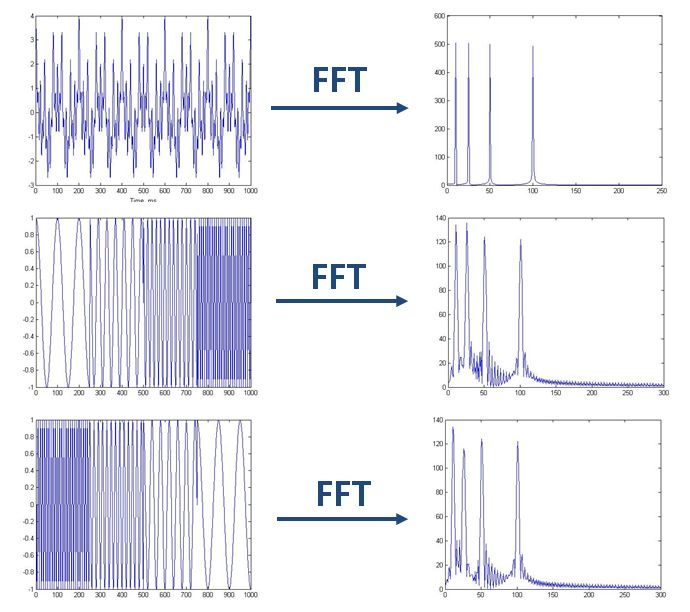
\includegraphics[scale=0.6]{non-stationary.jpg} 
%				\caption{平稳信号和非平稳信号及其傅里叶变换幅频特性} 
%				\label{stationary and non-stationary}
%			\end{figure}                
            

%			\begin{figure}[H]
%				\centering 
%				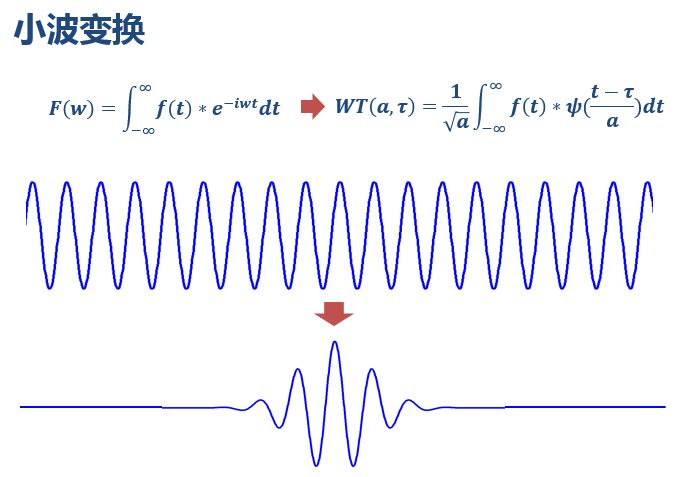
\includegraphics[scale=0.6]{wavelet-base.jpg} 
%				\caption{小波变换将无限长的三角函数基换成了有限长的小波基} 
%				\label{wavelet base}
%			\end{figure}            
            
 
 

        
% 
%                \begin{enumerate}[leftmargin=50pt]
%    				\item 输入一张低分辨率图像,得到其一组特征映射($feature\ maps$);
%    				\item 将得到的特征映射输入到一组子网中,用于预测出高分辨率图像的小波系数;
%    				\item 根据得到的小波系数重建出高分辨率图像。
%    			\end{enumerate}
                

            
%    			\begin{figure}[htbp]
%    				\centering 
%         			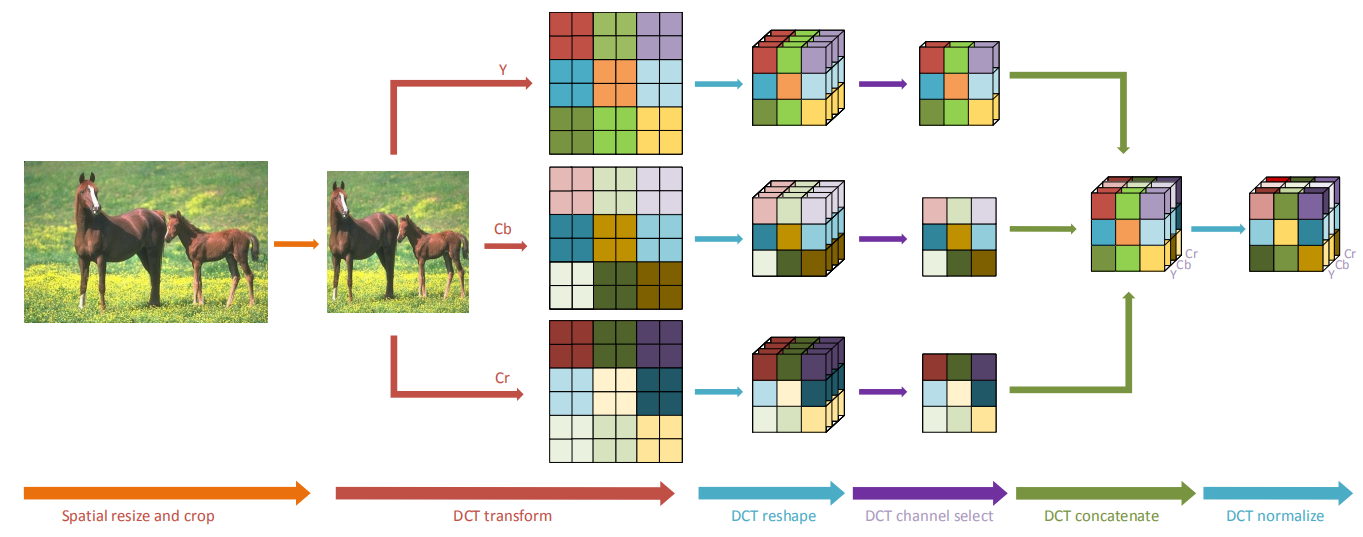
\includegraphics[scale=0.5]{pre-processing.png} 
%    				\caption{预处理流程示意图} 
%    				\label{pre-processing}
%    			\end{figure}
  
            
%        \nocite{digit_image_Gonzalez}
%        \nocite{signal_and_system}
%        \nocite{discrete-time_signal_processing}



		

            


%			\indent 采取\ref{数字相机成像原理}节的方式,我们也可以把线性扫描相机的原理概括为以下$3$个步骤:
%			\begin{enumerate}[leftmargin=50pt]
%				\item 由条带传感器成像,给出一幅图像一行(或一列)的像素值;
%				\item 沿垂直于传感器带的方向移动一小段距离;
%				\item 重复步骤$1$和步骤$2$,直至整幅图像全部成像完毕。
%			\end{enumerate}

%		\begin{enumerate}[leftmargin=50pt]
%			\item 所成图像在垂直方向上的大小不受限制;
%			\item 能够通过提高扫描频率达到非常高的分辨率;
%			\item 使用起来灵活方便等
%		\end{enumerate}
		
%	\section{实验验证}
%        \subsection{实验思想}
%            \indent 从前面的分析可以看出,频谱图上的谱线与空间域中像素变化的方向及剧烈程度有关。从这个角度出发,如果把空间域图像转一个角度,频谱图中的谱线相应地也应该旋转相同的角度。我们将在之后的两个小节中对这个猜想进行验证。
%        \subsection{实验代码}
%            	\begin{lstlisting}[language=Matlab,caption={实验代码},label={broadcast.cpp}]
%% reference: https://blog.csdn.net/jiugedexiaodi/article/details/79705308
%
%
%
%img = imread('C:\Users\Asus-\Desktop\数字图像\report\04\rotate45.png');
%img = rgb2gray(img);
%
%% 将图像的数据格式转换为double型的,此时图像的数值范围由原来的[0,255],
%% 变成了[0,1],其实不进行转换的话,也可以进行傅里叶变换,
%% 只是傅里叶变换后的图像会有所不同
%img=im2double(img);
%
%% size(img)
%
%F = fft2(img);
%F = fftshift(F);
%F = abs(F);
%
%% 傅里叶变换后模值差异非常大,低频直流远远大于高频
%% 不加这一句变换后的结果只能看到中间有一个亮点
%T = log(1+F);
%figure(1)
%subplot(1, 2, 1)
%imshow(img)
%subplot(1, 2, 2)
%% 后面的[],表示对图像做了一个类似于归一化的操作,
%% 防止傅里叶变换后模值差异太大
%imshow(T, [])
%            	\end{lstlisting}
                

        
%            \begin{figure}[htbp]
%            	\centering 
%                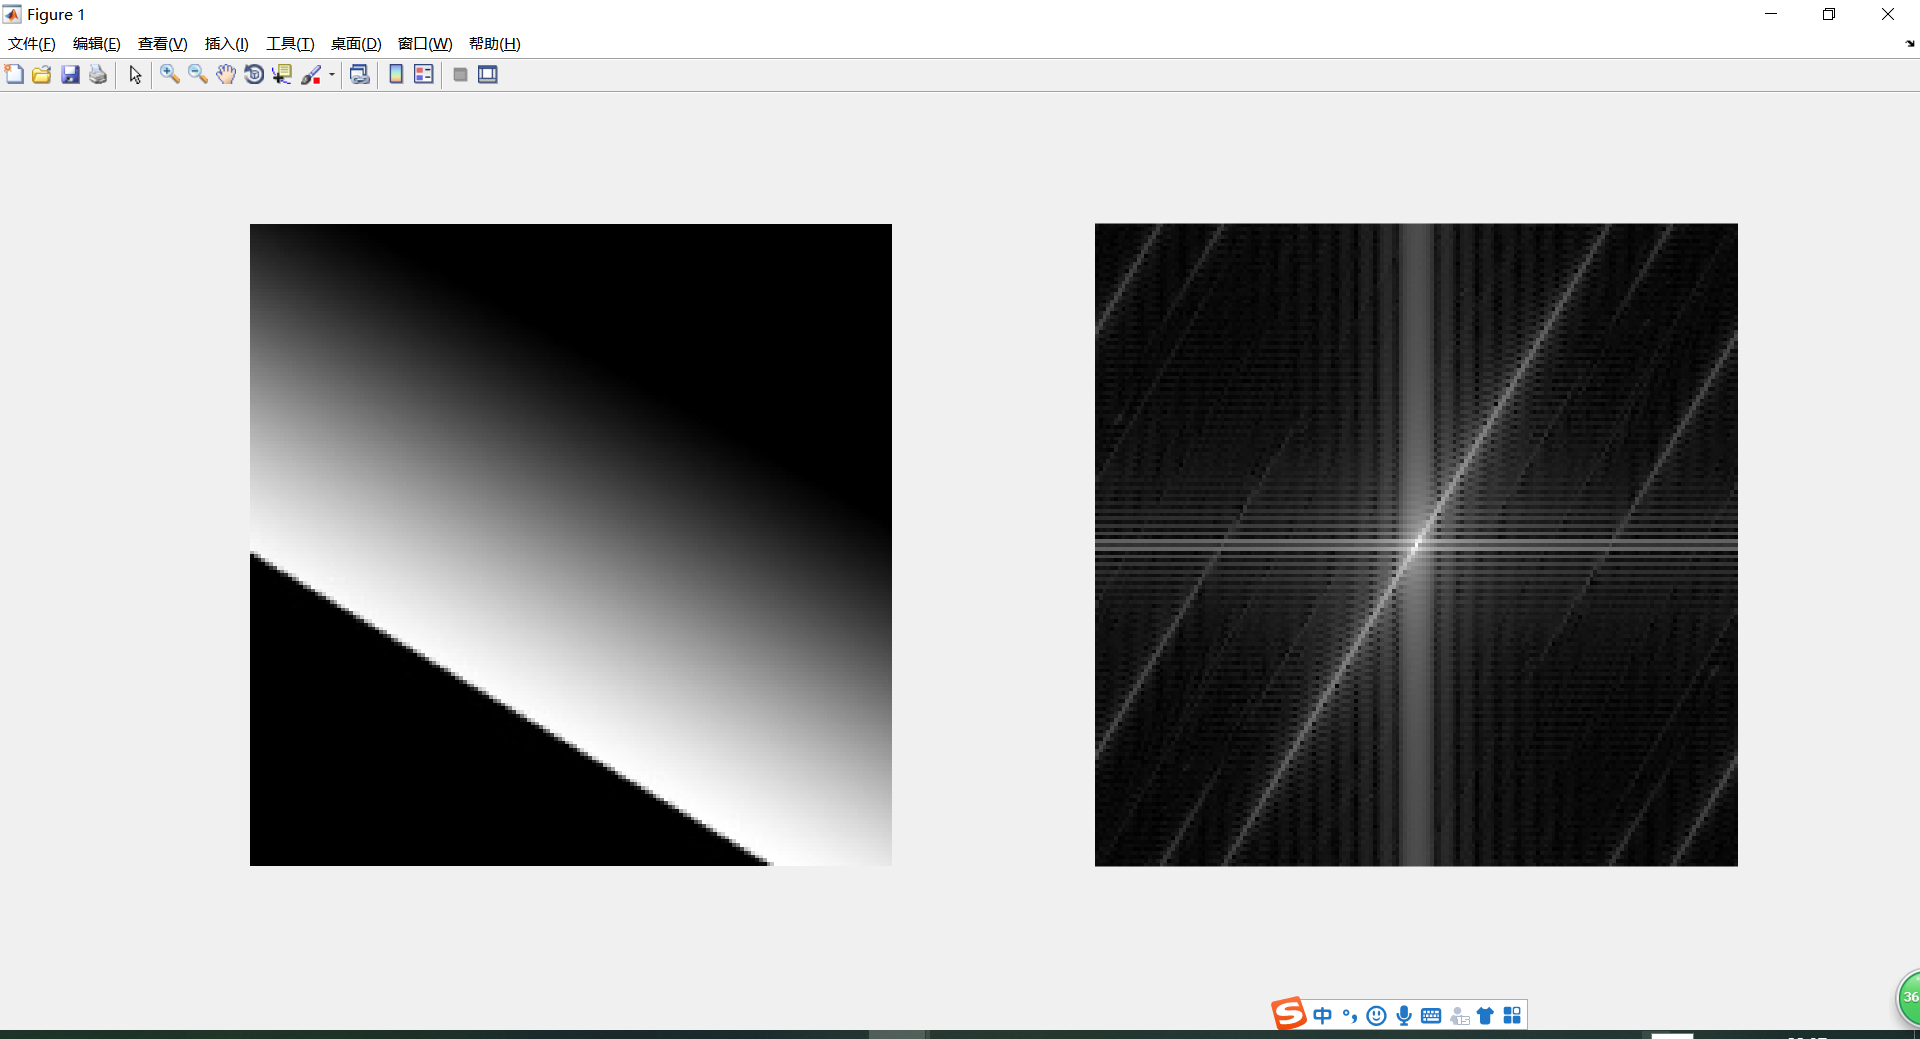
\includegraphics[scale=0.4]{result.png} 
%            	\caption{实验结果} 
%            	\label{result}
%            \end{figure}

            


	\section{总结}
        
        \indent 相比于如$JPEG2000$这样以$DCT$、$WT$为基础进行编码的的传统算法,深度学习更多依靠深度神经网络来实现编码器、解码器,经过训练达到一个较好的效果。同时,基于深度学习的图像很多时候是一个端到端的压缩模型,并不像$JPEG$、$JPEG2000$这样每一步都有着清晰的数学解释。但在部分文献(如\cite{Fu_2019_ICCV}中,也会将$DCT$与深度学习结合起来,以达到更好压缩效果,并取得更好的可解释性。
%			\begin{figure}[H]
%				\centering 
%				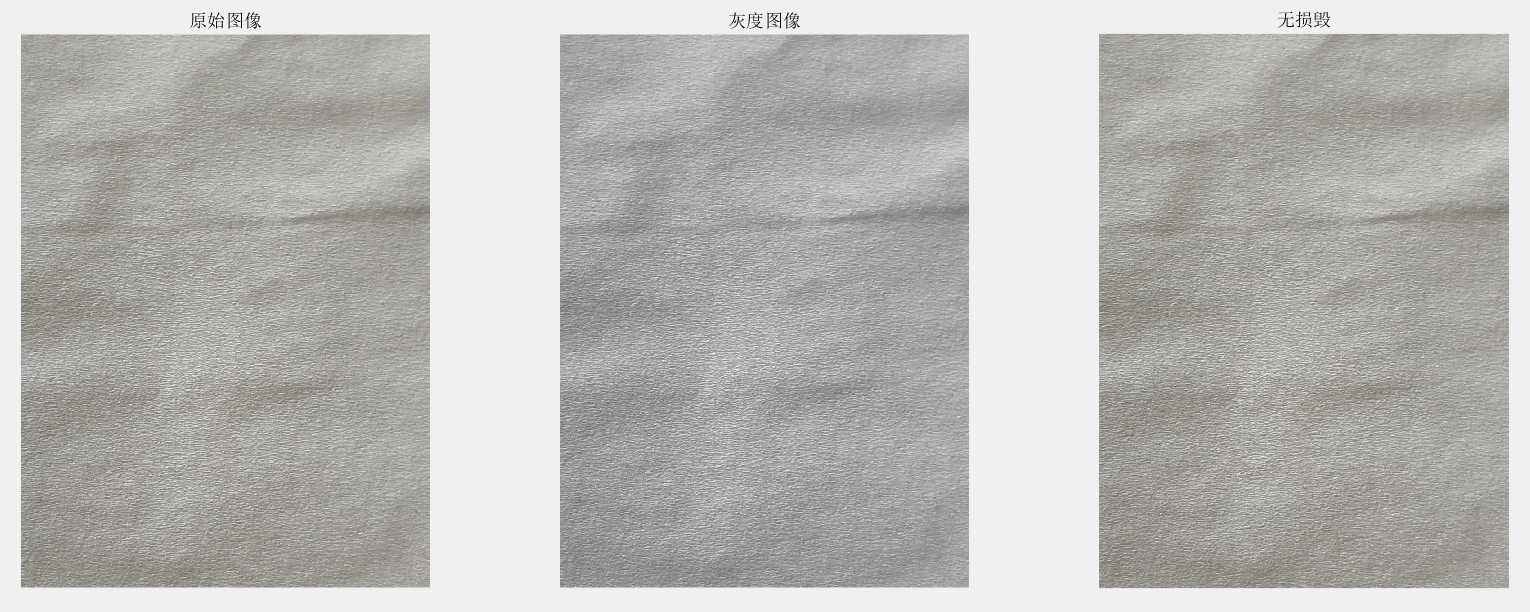
\includegraphics[scale=0.4]{res4.png} 
%				\caption{结果4} 
%				\label{res4}
%			\end{figure}
		

		
%			\begin{figure}[H]
%				\centering 
%				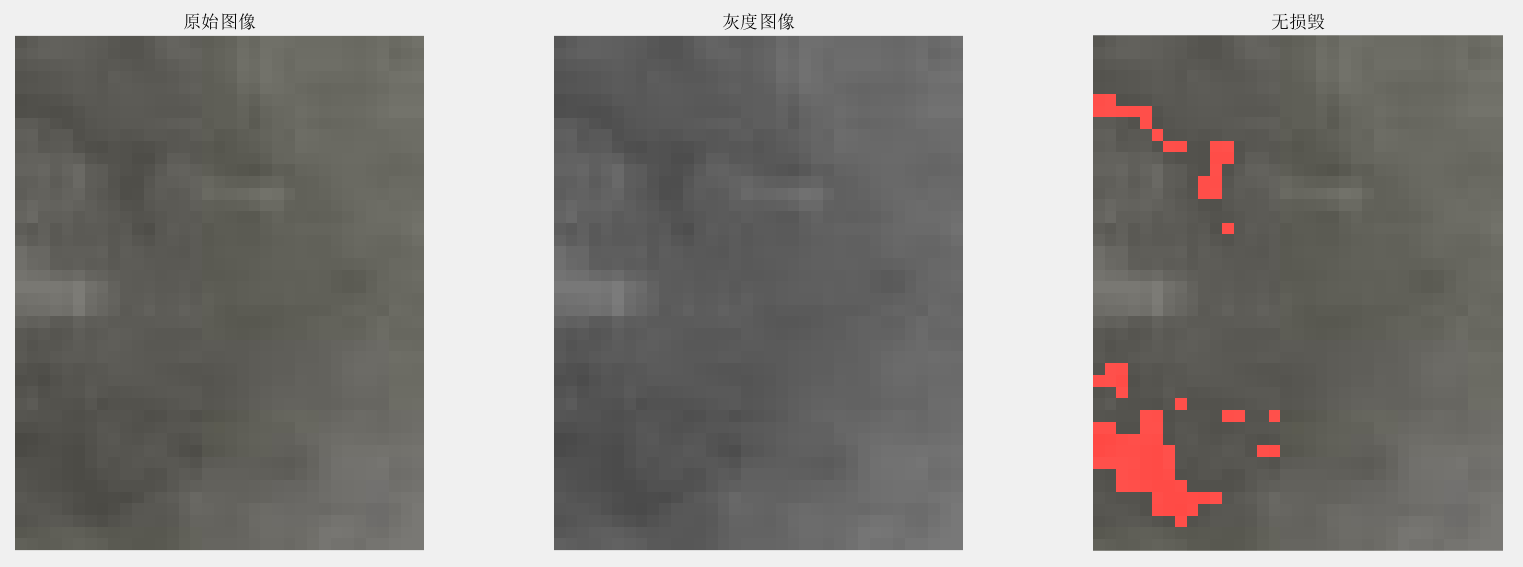
\includegraphics[scale=0.4]{res6.png} 
%				\caption{结果6(截取自结果5的阴影部分)} 
%				\label{res6}
%			\end{figure}
	
	
% 中文文献多个作者用中文逗号“,”连接
%\bibliography{ref.bib}
%\bibliographystyle{abbrv}
\bibliography{ref.bib}


\end{document}